%%%%%%%%%%%%%%%%%%%%%%%%%%%%%%%%%%%%%%%%%
% Lachaise Assignment
% LaTeX Template
% Version 1.0 (26/6/2018)
%
% This template originates from:
% http://www.LaTeXTemplates.com
%
% Authors:
% Marion Lachaise & François Févotte
% Vel (vel@LaTeXTemplates.com)
%
% License:
% CC BY-NC-SA 3.0 (http://creativecommons.org/licenses/by-nc-sa/3.0/)
% 
%%%%%%%%%%%%%%%%%%%%%%%%%%%%%%%%%%%%%%%%%

%----------------------------------------------------------------------------------------
%	PACKAGES AND OTHER DOCUMENT CONFIGURATIONS
%----------------------------------------------------------------------------------------

\documentclass[11pt]{article}

%%%%%%%%%%%%%%%%%%%%%%%%%%%%%%%%%%%%%%%%%
% Lachaise Assignment
% Structure Specification File
% Version 1.0 (26/6/2018)
%
% This template originates from:
% http://www.LaTeXTemplates.com
%
% Authors:
% Marion Lachaise & François Févotte
% Vel (vel@LaTeXTemplates.com)
%
% License:
% CC BY-NC-SA 3.0 (http://creativecommons.org/licenses/by-nc-sa/3.0/)
% 
%%%%%%%%%%%%%%%%%%%%%%%%%%%%%%%%%%%%%%%%%

%----------------------------------------------------------------------------------------
%	PACKAGES AND OTHER DOCUMENT CONFIGURATIONS
%----------------------------------------------------------------------------------------

\usepackage{amsmath,amsfonts,stmaryrd,amssymb} % Math packages

\usepackage{enumerate} % Custom item numbers for enumerations

\usepackage[ruled]{algorithm2e} % Algorithms
\usepackage{listings}
\usepackage{graphicx}
\usepackage{subcaption}
\usepackage{booktabs}
\usepackage[ngerman,english]{babel}
\usepackage{graphicx}
\usepackage{flafter}
\usepackage{placeins}
\usepackage[mediumspace,mediumqspace,Grey,squaren]{SIunits}
\usepackage{amsmath}
\usepackage{color}

\usepackage{relsize}
\usepackage[table,xcdraw]{xcolor}
\usepackage{amsmath}
\usepackage{textcomp}
\usepackage{mathtools}
\usepackage{hyperref}
\usepackage{subcaption}
\usepackage[framemethod=tikz]{mdframed} % Allows defining custom boxed/framed environments

\usepackage{listings} % File listings, with syntax highlighting
\lstset{
	basicstyle=\ttfamily, % Typeset listings in monospace font
}

\newcolumntype{s}{>{\columncolor[HTML]{AAACED}} p{3cm}}
\newcolumntype{?}{!{\vrule width 2pt}}


%----------------------------------------------------------------------------------------
%	DOCUMENT MARGINS
%----------------------------------------------------------------------------------------

\usepackage{geometry} % Required for adjusting page dimensions and margins

\geometry{
	paper=a4paper, % Paper size, change to letterpaper for US letter size
	top=2.5cm, % Top margin
	bottom=3cm, % Bottom margin
	left=2.5cm, % Left margin
	right=2.5cm, % Right margin
	headheight=14pt, % Header height
	footskip=1.5cm, % Space from the bottom margin to the baseline of the footer
	headsep=1.2cm, % Space from the top margin to the baseline of the header
	%showframe, % Uncomment to show how the type block is set on the page
}

%----------------------------------------------------------------------------------------
%	FONTS
%----------------------------------------------------------------------------------------

\usepackage[utf8]{inputenc} % Required for inputting international characters
\usepackage[T1]{fontenc} % Output font encoding for international characters

\usepackage{XCharter} % Use the XCharter fonts

%----------------------------------------------------------------------------------------
%	COMMAND LINE ENVIRONMENT
%----------------------------------------------------------------------------------------

% Usage:
% \begin{commandline}
%	\begin{verbatim}
%		$ ls
%		
%		Applications	Desktop	...
%	\end{verbatim}
% \end{commandline}

\mdfdefinestyle{commandline}{
	leftmargin=10pt,
	rightmargin=10pt,
	innerleftmargin=15pt,
	middlelinecolor=black!50!white,
	middlelinewidth=2pt,
	frametitlerule=false,
	backgroundcolor=black!5!white,
	frametitle={Command Line},
	frametitlefont={\normalfont\sffamily\color{white}\hspace{-1em}},
	frametitlebackgroundcolor=black!50!white,
	nobreak,
}

% Define a custom environment for command-line snapshots
\newenvironment{commandline}{
	\medskip
	\begin{mdframed}[style=commandline]
}{
	\end{mdframed}
	\medskip
}

%----------------------------------------------------------------------------------------
%	FILE CONTENTS ENVIRONMENT
%----------------------------------------------------------------------------------------

% Usage:
% \begin{file}[optional filename, defaults to "File"]
%	File contents, for example, with a listings environment
% \end{file}

\mdfdefinestyle{file}{
	innertopmargin=1\baselineskip,
	innerbottommargin=0.6\baselineskip,
	topline=false, bottomline=false,
	leftline=false, rightline=false,
	leftmargin=0cm,
	rightmargin=0cm,
	singleextra={%
		\draw[fill=black!10!white](P)++(0,-1.2em)rectangle(P-|O);
		\node[anchor=north west]
		at(P-|O){\ttfamily\mdfilename};
		%
		\def\l{3em}
		\draw(O-|P)++(-\l,0)--++(\l,\l)--(P)--(P-|O)--(O)--cycle;
		\draw(O-|P)++(-\l,0)--++(0,\l)--++(\l,0);
	},
	nobreak,
}

% Define a custom environment for file contents
\newenvironment{file}[1][File]{ % Set the default filename to "File"
	\medskip
	\newcommand{\mdfilename}{#1}
	\begin{mdframed}[style=file]
}{
	\end{mdframed}
	\medskip
}

%----------------------------------------------------------------------------------------
%	NUMBERED QUESTIONS ENVIRONMENT
%----------------------------------------------------------------------------------------

% Usage:
% \begin{question}[optional title]
%	Question contents
% \end{question}

\mdfdefinestyle{question}{
	innertopmargin=1.2\baselineskip,
	innerbottommargin=0.8\baselineskip,
	roundcorner=5pt,
	nobreak,
	singleextra={%
		\draw(P-|O)node[xshift=1em,anchor=west,fill=white,draw,rounded corners=5pt]{%
		question \theQuestion\questionTitle};
	},
}

\newcounter{Question} % Stores the current question number that gets iterated with each new question

% Define a custom environment for numbered questions
\newenvironment{question}[1][\unskip]{
	\bigskip
	\stepcounter{Question}
	\newcommand{\questionTitle}{~#1}
	\begin{mdframed}[style=question]
}{
	\end{mdframed}
	\medskip
}

%----------------------------------------------------------------------------------------
%	WARNING TEXT ENVIRONMENT
%----------------------------------------------------------------------------------------

% Usage:
% \begin{warn}[optional title, defaults to "Warning:"]
%	Contents
% \end{warn}

\mdfdefinestyle{warning}{
	topline=false, bottomline=false,
	leftline=false, rightline=false,
	nobreak,
	singleextra={%
		\draw(P-|O)++(-0.5em,0)node(tmp1){};
		\draw(P-|O)++(0.5em,0)node(tmp2){};
		\fill[black,rotate around={45:(P-|O)}](tmp1)rectangle(tmp2);
		\node at(P-|O){\color{white}\scriptsize\bf !};
		\draw[very thick](P-|O)++(0,-1em)--(O);%--(O-|P);
	}
}

% Define a custom environment for warning text
\newenvironment{warn}[1][Warning:]{ % Set the default warning to "Warning:"
	\medskip
	\begin{mdframed}[style=warning]
		\noindent{\textbf{#1}}
}{
	\end{mdframed}
}

%----------------------------------------------------------------------------------------
%	INFORMATION ENVIRONMENT
%----------------------------------------------------------------------------------------

% Usage:
% \begin{info}[optional title, defaults to "Info:"]
% 	contents
% 	\end{info}

\mdfdefinestyle{info}{%
	topline=false, bottomline=false,
	leftline=false, rightline=false,
	nobreak,
	singleextra={%
		\fill[black](P-|O)circle[radius=0.4em];
		\node at(P-|O){\color{white}\scriptsize\bf i};
		\draw[very thick](P-|O)++(0,-0.8em)--(O);%--(O-|P);
	}
}

% Define a custom environment for information
\newenvironment{info}[1][Info:]{ % Set the default title to "Info:"
	\medskip
	\begin{mdframed}[style=info]
		\noindent{\textbf{#1}}
}{
	\end{mdframed}
}
 % Include the file specifying the document structure and custom commands

%----------------------------------------------------------------------------------------
%	ASSIGNMENT INFORMATION
%----------------------------------------------------------------------------------------

\title{MMD: Programming Assignment \#1}
\author{Group 1:~ E. Guliev, J. Rass, C. Wiskott}
   %Matr.Nr.: 15 07 006, 15 04 276 ,15 05 394

  

\date{University of Vienna --- \today} % University, school and/or department name(s) and a date

%----------------------------------------------------------------------------------------

\begin{document}
\maketitle 

\begin{abstract}
All tasks were completed and instructions on executing the program can be found in the attached \texttt{README.txt}. Furthermore they are uploaded to the GitHub repository: \url{https://github.com/ezorrio/genre-classification}. The files require no input parameters and can simply be run with a standard IDE or from the command-line. The print statements produce the relevant results.

Data is stored on Github using LFS \url{https://git-lfs.github.com}. If you have all needed data - FMA dataset, you can clone the repository without downloading them by using 
\begin{lstlisting}
GIT_LFS_SKIP_SMUDGE=1 git clone
https://github.com/ezorrio/genre-classification
\end{lstlisting}


The best achieved results on the validation set are around 45\% while the accuracy on the test set is around 33\%.



\end{abstract}

\section*{Local Sensitive Hashing (LSH) for Item Search}

The goal of this assignment was to implement an efficient nearest neighbor algorithm for genre classification of previously unclassified music tracks. For this purpose we used LSH as a framework for the similar item search while incorporating the random projection method. The sought-for result was a classification model that, given the optimal hyper-parameters obtained trough careful testing, would return a reasonable classification score for the provided test set and thus would be able to autonomously classify new music tracks. 

\section*{Implementation}

\subsection*{Subtask 1: Data Loading and Data Preparation}

\begin{file}[FMA-Class]
\begin{lstlisting}[language=Python]
class FMA:
    def __init__(self, path, subset='small',
                 feature_fields=None)
\end{lstlisting}
\end{file}
The data used for this experiment stems from the Free Music Archive (FMA)\footnote{\url{https://github.com/mdeff/fma}} and uses the \texttt{fma\_metadata.zip} files. Out of those files \texttt{tracks.csv} and \texttt{features.csv} are considered for the training and verification process. For both data sets the \texttt{'small'} subset is considered which contains 8000 samples over 8 different genres with varying representation over the whole set. To ensure a good split of the data for training purposes, the pre defined splits \texttt{'training' (6400 samples), 'validation' (800 samples), 'test (800 samples)'} are used, which are already set up in a stratified way where each genre is represented with the same amount of samples. The data is loaded into the \texttt{FMA} class and processed according to the parameters given in the main program. For training a combination of feature sets of the \texttt{features.csv} file various combinations of the available feature sets are considered, but after a lengthy testing period the \texttt{'mfcc'} feature set proved to deliver the best results.

\subsection*{Subtask 2: RandomHash}
The random hashes are generated by using randomly generated projection matrices with the condition
\begin{align*}
r_{i,j} = \sqrt{3} \cdot \left\{\begin{matrix}
+1 & with\,probability\,\frac{1}{6}\\ 
0 & with\,probability\,\frac{2}{3}\\ 
-1 & with\,probability\,\frac{1}{6}
\end{matrix}\right.
\end{align*}

using the \texttt{RandomHash} class.

\begin{file}[RandomHash-Class]
\begin{lstlisting}[language=Python]
class RandomHash:
    def __init__(self, data_size, hash_length)
\end{lstlisting}
\end{file}

The class itself takes the number of features and the length of the hash value as inputs and generates the random projection matrix using the above displayed condition. The number of generated projection matrices is decided by the user using the \texttt{LSH} class, where the incoming samples get multiplied with the random projection matrices to generate hash values for the buckets. The approach of using random projections is used as a simple method of converting data in high dimensional space into a lower dimensional one. The specific method in this case is used, because it produces a uniform distribution of vectors into space with mean 0 and variance 1, which is desirable for approximated nearest neighbour algorithms, while also keeping the computational cost very low compared to generating these vectors with a Gaussian distribution methods. Furthermore this class is used to calculate the hash values, add them to their respective bucket, and retrieve them for given input data.

\subsection*{Subtask 3: LSH}

\begin{file}[LSH-Class]
\begin{lstlisting}[language=Python]
class LSH:
    def __init__(self, data_size, hashes_count, hash_length)
\end{lstlisting}
\end{file}

The \textit{LSH} class functions as the container for the different hash tables i.e. the objects of the class \textit{RandomHash}, each  containing hash values and their corresponding track ids. The argument \textit{hashes\_count} regulates the amount of hash tables and the \textit{hash\_length} the length of the hash keys in every hash table.

The \textit{hash\_data} function takes a data set, iterates through all feature vectors and passes the vectors and their corresponding track ids to all hash tables contained in\textit{ self.hashes }i.e. builds the hash tables from the given data, which is done during the training phase of the algorithm.

The \textit{get} function takes a feature vector and is used to obtain all track ids from each hash table that share the same hash key as the hashes feature vector. 

\subsection*{Subtask 4: MusicSearch}

Using the implementation of the blog-post as a template, we created the class \textit{MusicSearch} in order to carry out the approximated k-nearest-neighbor (\textit{knn}) search. It takes the parameters \textit{n} (number of hash tables), \textit{l} (hash length), the FMA data-subset, the subset of the features, the similarity measure,\textit{ k} (number of neighbors to consider in knn) as well as the metric \textit{"magic number"}, which regulates the size of the random subset of similar tracks in the course of the genre prediction.
The class features a set of standard train functions that utilize the\textit{ LSH.hash\_data} method to build the hash tables from the training data as well as test-functions that are used during the evaluation phase. 

\begin{file}[MusicSearch-Class]
\begin{lstlisting}[language=Python]
class MusicSearch:
    def __init__(self, data_path, n, l, subset='small', 
    feature_fields=None, measure='Cosine', k=5, 
    magic_number=800)
\end{lstlisting}
\end{file}


The rest of the functions revolve around the knn-problem, starting with computing the similar tracks via the \textit{find\_similar\_tracks}-function, which takes a feature vector as an argument, hashes it to every hash table and returns the track ids with the same hash key. Because, in some cases, the amount of similar tracks are in the thousands, the problem was approximated by only taking a subset of similar tracks (see the \textit{k\_neighbors}-function). The size of this subset was jokingly called "\textit{magic\_number}", due to the enormous effect it has on the run-time as well as the classification score. With the smaller subset, the run-time of the genre classification for the "small" FMA data-set, was reduced by a factor of up to 5, while reducing the accuracy only by around 2-4\%, thus constituting a sensible trade-off for this problem. \\

After selecting the subset, the pairwise similarities of the feature vector and the feature vectors of the similar tracks are calculated, which are then  sorted according to the chosen similarity measure. Only the track ids of the k-most similar tracks are returned, which are then used to compute the most similar genre. This genre is finally taken as the predicted genre of the given feature vector.  
In the case,  that less than k similar tracks are found for a given feature vector, the algorithm calculates the most common genre of however many similar tracks were found.

The genre classification for the entire test set culminates in the \textit{print\_classification\_results}-function which prints the classification score for each genre as well as the overall i.e. average classification score over all genres. 









\section*{Training}

\subsection*{Parameters and their definition}
In order to speed-up the calculation, instead of comparing given element with every single item in hashtables, we pick up maximum this amount of items in a random way
\begin{table*}[htb]
\begin{center}
\resizebox{\textwidth}{!}{%
\begin{tabular}{|l|l|}
\hline
\textbf{Parameter}              & \textbf{Description}                                                      \\ \hline
\textit{number\_of\_hashtables} & Defines the amount of hashtables within LSH model                         \\ \hline
\textit{hash\_length}           & Size of hash                                                              \\ \hline
\textit{subset}        & Data subset to work on. Related to FMA. Fixed to small.                   \\ \hline
\textit{feature\_fields}        & A list of features we want to count during model training                 \\ \hline
\textit{measure}                & Used to calculate similarity between features. Can be Euclidian or Cosine \\ \hline
\textit{k}                      & Parameter for KNN search                                                  \\ \hline
\textit{magic\_number} &
  \begin{tabular}[c]{@{}l@{}}In order to speed-up the calculation, \\instead of comparing given element with every single item in hashtables, \\ we pick up maximum this amount of items in a random way\end{tabular} \\ \hline
\end{tabular}%
}
\caption{Parameters description}
\end{center}
\end{table*}

\subsection*{Automatic execution}

In order to understand the behavior and the way each parameters affect the accuracy of the model, we have written a small script to evaluate different combinations of above-mentioned parameters.

1. While inspecting execution logs, it was quite clear that among of all feature combinations tested, best value for \textit{feature\_field} = "mfcc".

2. Furthermore, according to those logs it was also clear that with increasing k we overall get better models

\begin{table*}[htb]
\begin{center}
\begin{tabular}{|l|l|}
\hline
\textbf{K}          & \textbf{Amount of models with accuracy >= 40\%}                             
\\ \hline
\textit{3}          & 1                         
\\ \hline
\textit{5}          & 4                                                              
\\ \hline
\textit{7}          & 8            
\\ \hline
\end{tabular}%
\caption{Correlation of k with quality}
\end{center}
\end{table*}

3. In most cases increasing \textit{magic\_number} improves accuracy

4. We have 13 models with accuracy of more than 40\%. 6 of them use Cosine as distance measure, 7 - Euclidean.

5. Best genre accuracy gained among those models - Folk: 70\%. Worst - Experimental: 9\%

6. Best overall accuracy among all the models - 41\%. 

\subsection*{Manual tuning}

Experiments from previous section helped us to get a little bit of insight of how each parameter affects our model.
Based on that knowledge, we can fix following parameters:

\begin{table*}[htb]
\begin{center}
\begin{tabular}{|l|l|}
\hline
\textbf{Parameter}              & \textbf{Value}                                                      
\\ \hline
\textit{feature\_fields}        & ["mfcc"]                 
\\ \hline
\textit{measure}                & Cosine 
\\ \hline
\textit{magic\_number}          & As much as possible (keep in mind runtime)
\\ \hline
\end{tabular}
\caption{Fixed parameters and their values}
\end{center}
\end{table*}

Therefore, \textit{k}, \textit{number\_of\_hashtables} and \textit{hash\_length} parameters left and are subject of experiments further.

As a starting point, we took best model (accuracy-wise) from automatic executions. Magic number is set to 1500
Below steps taken for parameters optimization are provided:

\begin{table*}[htb]
\begin{center}
\begin{tabular}{|l|l|l|l|l|l}
\hline
\textbf{Step №} & \textbf{k} & \textbf{number\_of\_hashtables} & \textbf{hash\_length} & \textbf{Accuracy} & \textbf{Notes}      
\\ \hline
1.              & 7          & 20                              & 16                    & 42.5\%            &             
\\ \hline
2.              & 10         & 20                              & 16                    & 43.125\%          &            
\\ \hline
3.              & 15         & 20                              & 20                    & 44\%              &       
\\ \hline
4.              & 15         & 25                              & 20                    & 42.375\%          & Failed. Restore to 3.     
\\ \hline
5.              & 15         & 20                              & 25                    & 45.125\%          &       
\\ \hline
6.              & 20         & 20                              & 25                    & 46\%              &       
\\ \hline
7.              & 20         & 25                              & 25                    & 45.625\%          & Failed. Restore to 6.    
\\ \hline

\end{tabular}%
\caption{Manual optimization steps}
\end{center}
\end{table*}

\newpage
So far best result was gained within experiment 6. Let us use that for evaluation of the model with \textit{magic\_number}=8000. Instead of picking subset of items to compare with it will use the all the items available, thus using KNN instead of aKNN.

\begin{figure}[ht]
    \begin{centering}
        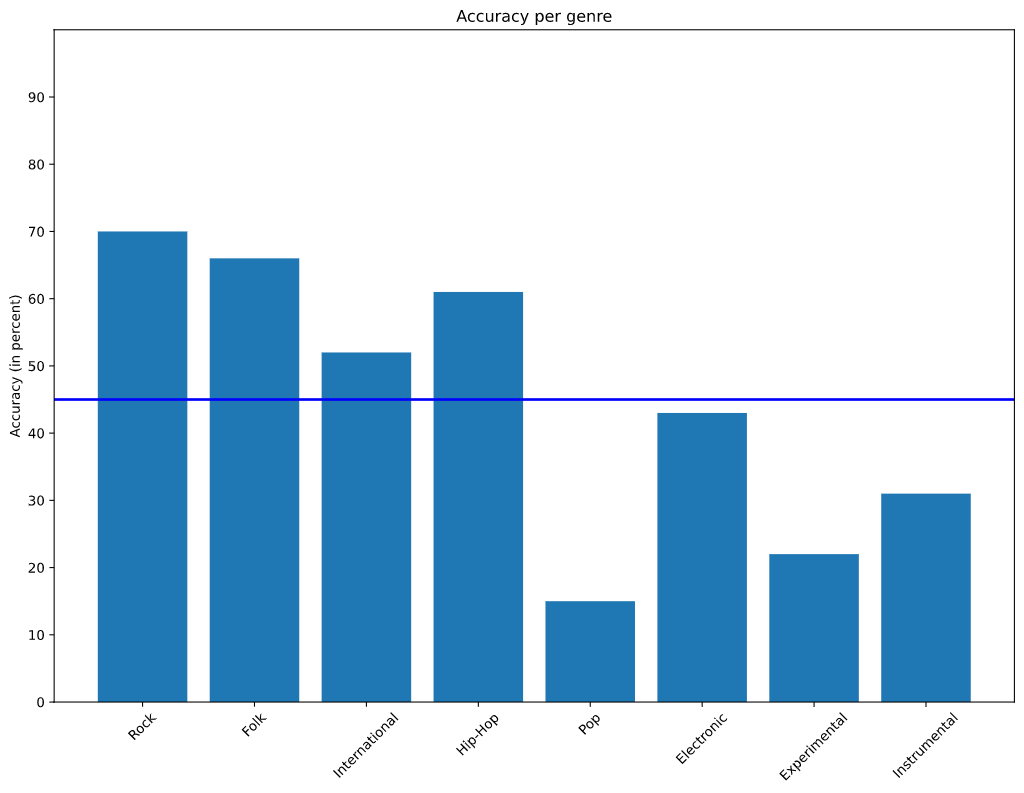
\includegraphics[width=0.75\textwidth]{Training vs validation.png}
 	    \caption{Training vs Validation Data}
 	    {\small  }
        \label{Fig:1}  
    \end{centering}
\end{figure}

Definitely there is possibility that we can pick up better hyperparameters, but result of 45\% is pretty acceptable: as we have 8 genres, training\/validation\/test data in uniformly distributed among genres, the probability of randomly predicting the correct genre is $\frac{1}{8}$=12.5\% which is much less than 45\%, so model definitely works as needed.

Additionally it is worth to mention that all evaluations were done on validation set, such that we don't know yet how will it work of the test data.

\subsection*{Evaluating test data}

For that purpose we will use the best model gained from the previous section, combine train the model on training/training and validation sets combined, and evaluate against test set.

\begin{figure}[ht]
    \begin{centering}
        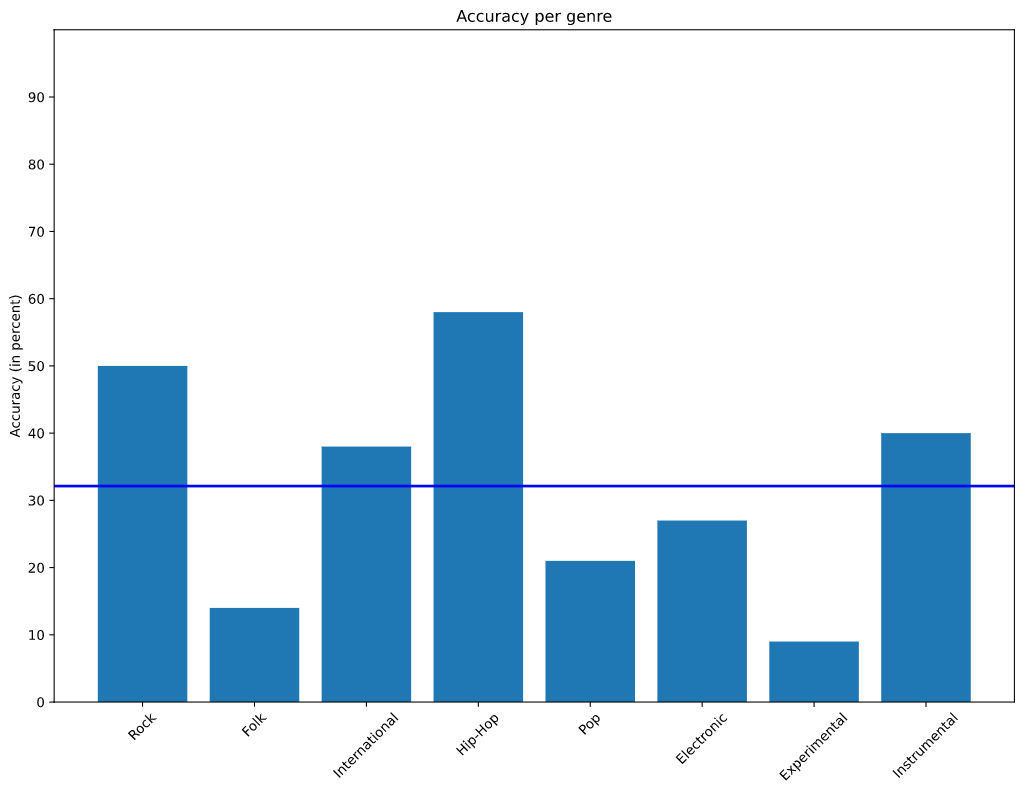
\includegraphics[width=0.75\textwidth]{Training vs test.png}
 	    \caption{Training vs Test Data}
 	    {\small  }
        \label{Fig:2}  
    \end{centering}
\end{figure}

\begin{figure}[ht]
    \begin{centering}
        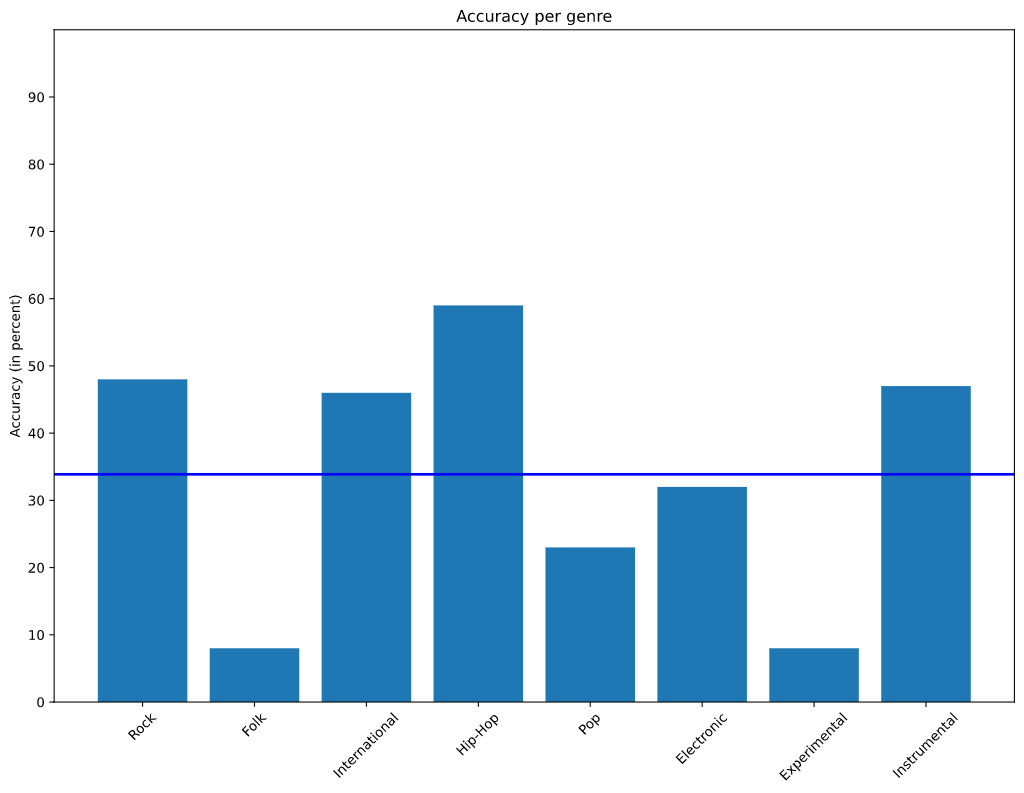
\includegraphics[width=0.75\textwidth]{Training and validation vs test.png}
 	    \caption{Training and Validation vs Test Data}
 	    {\small  }
        \label{Fig:3}  
    \end{centering}
\end{figure}
\clearpage

When evaluating against the final testing data the model trained on the only the training data and accuracy of 32.125\% is achieved, while the model trained on the training and validation data achieves an accuracy of 33.875\% with the following hyperparameters.

\begin{table*}[h]
\begin{center}

\begin{tabular}{|l|l|}
\hline
\textbf{Parameter}              &         \textbf{Value}                  \\ \hline
\textit{number\_of\_hashtables} & 20                         \\ \hline
\textit{hash\_length}           & 25                                                              \\ \hline
\textit{subset}        & small                   \\ \hline
\textit{feature\_fields}        & mfcc                 \\ \hline
\textit{measure}                & Cosine \\ \hline
\textit{k}                      & 20                                                 \\ \hline
\textit{magic\_number} &    8000 \\ \hline
\end{tabular}%

\caption{Parameters used for runs against test data}
\end{center}
\end{table*}

\section*{Contributions}

The tasks and corresponding contributions from each member are listed below.

\begin{table}[h]
\begin{tabular}{llll}
Task                                               & E. Guliev                 & J. Rass                   & C. Wiskott                \\ \hline
Initial Project Setup                              & \checkmark & \checkmark & \checkmark \\
Task distribution planning                         & \checkmark & \checkmark & \checkmark \\
Data exploration                                   & \checkmark & \checkmark & \checkmark \\
Initial Draft Version                              & \checkmark & \checkmark & \checkmark \\
Merging the solutions                              & \checkmark & \checkmark & \checkmark \\
Global refractor, splitting algorithm into classes & \checkmark & \checkmark & \checkmark \\
Execution, Optimizing parameters                   & \checkmark & \checkmark & \checkmark \\
Testing, Evaluating accuracy                       & \checkmark & \checkmark & \checkmark \\
Report                                             & \checkmark & \checkmark & \checkmark
\end{tabular}
\end{table}

Every team member tried to develop their own version as an initial draft, which got merged together to form the final algorithm. Testing the hyperparameters was also split up between the team members to split up the run time for validating the parameters.

% \begin{figure}[ht]
% 	\includegraphics[width=\textwidth]{2.png}
% 		\caption[1.1]
% 		{\small  }
% 	\label{Fig:2}
% \end{figure}

% \begin{table}[h!]
%   \begin{center}
%     \label{tab:results}
%     \begin{tabular}{l|c|c|c?c}
%       \toprule % <-- Toprule here
%       \textbf{n} & \textbf{l} & \textbf{k} & \textbf{m} & \textbf{Score [\%]}\\
%       \midrule % <-- Midrule here
%       5 & 12 & 5 & Cosine & \cellcolor[HTML]{FFBF00} 29.7 \\ % color could be used to mark best classification score or the entire row
%       &  & \\
%       & & \\
%       \bottomrule % <-- Bottomrule here
%     \end{tabular}
%         \caption{Results of genre classification applied to the validation set using different combinations of hyper-parameters.}
%   \end{center}
% \end{table}

% \section*{Conclusion}



%----------------------------------------------------------------------------------------

\end{document}
